\chapter{Simulations}
\section{Introduction}
Dans ce chapitre, nous allons explorer les performances des méthodes d'estimation de la ddp non paramétriques en utilisant des données simulées à partir de lois usuelles telles que la loi normale, la loi exponentielle et la loi uniforme. L'objectif de cette simulation est d'évaluer les performances de différentes méthodes d'estimation de la ddp et de comparer les résultats avec les vraies valeurs de la ddp.
Nous allons d'abord présenter les lois usuelles que nous allons simuler, notamment la loi normale et la loi exponentielle. Nous allons ensuite expliquer comment nous avons simulé ces lois à partir de données aléatoires. Nous allons ensuite utiliser des méthodes d'estimation de la ddp non paramétriques pour estimer la ddp des données simulées. Nous allons évaluer les performances de ces méthodes en utilisant EQM et les comparer avec les vraies valeurs de la ddp.
Cette simulation est importante car elle permettra de déterminer la performance des différentes méthodes d'estimation de la ddp non paramétriques dans des situations contrôlées. Les résultats de cette simulation pourront ensuite être généralisés à des situations plus complexes et réelles. Cette simulation est également importante car elle peut aider à comprendre les avantages et les limites des différentes méthodes d'estimation de la ddp non paramétriques. Ces informations peuvent être utiles pour choisir la méthode la plus appropriée dans différentes situations d'analyse de données.
En conclusion, ce chapitre de simulation permettra d'évaluer les performances des méthodes d'estimation de la ddp non paramétriques à partir de données simulées. Nous espérons que les résultats de cette simulation pourront fournir des informations utiles sur les performances des différentes méthodes d'estimation de la ddp et aider à choisir la méthode la plus appropriée dans différentes situations d'analyse de données.
\newpage

\section{Description des lois utilisées}
Nous avons procédé à des simulations sur différentes lois de probabilité, à savoir:
\newline 
\newline    
\begin{itemize}
   \item[$\bullet$] Une densité de probabilité, en l'occurrence une \textbf{loi normale}.\\
   \begin{lstlisting}
    import numpy as np
    #m Moyenne
    #s ecart-type
    #n taille echantillon
def generation_LN(m, s, n):
    mln = np.zeros(n)
    LN = np.random.randn(n)
    for i in range(n):
        LN[i] = m + s * LN[i]
    return(LN)

    \end{lstlisting}

    \vspace{1.5cm}
       \item[$\bullet$] Une densité de probabilité mixte(combinée), en l'occurrence une \textbf{loi exponentielle} et une \textbf{loi normale}.\\
   \begin{lstlisting}
    def generation_Mix(lam,mu,sigma,n_samples):
    #m Moyenne
    #sigma Ecart-type
    #lam Lambda
    #n_samples Taille echantillon
    samples = np.zeros(n_samples)
    for i in range(n_samples):
        if np.random.uniform() < lam:
            samples[i] = np.random.exponential(scale=1/lam)
        else:
            samples[i] = np.random.normal(loc=mu, scale=sigma)
            
    return(samples) 
    \end{lstlisting}

           \item[$\bullet$] Une densité de probabilité, en l'occurrence une \textbf{loi uniforme},\\ à savoir une loi uniforme entre $] a ,b [$.\\
           
   \begin{lstlisting}
    import numpy as np
def generation_LE(a,b,n):

    LE = np.random.uniform(low=a, high=b, size=n)

    return(LE)

    \end{lstlisting}
    \vspace{0.5cm}
\end{itemize}

Durant ces simulations nous comparer les performances des méthodes de noyau et de l’histogramme. Pour la méthode de noyau nous allons également comparer les performances en faisant varier les méthodes d’optimisation du paramètre de lissage.
\vspace{0.25cm}
\begin{itemize}
   \item[$\bullet$]\textbf{Histogramme} :\\
   Les étapes comprennent la division de l'intervalle des données en bins (classes), le calcul de la fréquence dans chaque bin, et la normalisation des fréquences pour obtenir une estimation graphique de la ddp de l'échantillon de données.
En ce qui concerne l’optimisation de $h_N$ nous allons suivre cette méthode \shortcite{freedman1981histogram} :
$$
\begin{aligned}
n_{\text{I}} &= \left\lfloor n^{1/3} \right\rfloor \\
h_N &= \frac{a-b}{n_{\text{I}}} \\
\text{avec } \text{A} &= \{a_1, a_2, \ldots, a_n\} \\
a &= \max\{a_1, a_2, \ldots, a_n\} \\
b &= \min\{a_1, a_2, \ldots, a_n\} \\
\left\lfloor x \right\rfloor &= \max\{n \in \mathbb{Z} \mid n \leq x\}
\end{aligned}
$$
 \item[$\bullet$]\textbf{Noyau - ROT} :\\Cette méthode est prédéfinie en Python 3, donc va appeler la méthode adéquate directement. 
 \item[$\bullet$]\textbf{Noyau - LSCV} :\\Cette méthode utilise l’estimateur à noyau avec recherche du pas optimal en utilisant la classe GridSearchCV de la bibliothèque scikit-learn.  
 \item[$\bullet$]\textbf{Noyau - PlugIn} :\\Cette méthode utilise l’estimateur à noyau avec recherche du pas optimal en l’algorithme Plug-In 

   
\end{itemize}
\newpage
Comme métrique d’évaluation de performance, Nous avons opté pour EQM, c’est une mesure couramment utilisée pour évaluer la qualité d'une méthode d’estimation de probabilité, en calculant la moyenne des carrés des différences entre les densités estimées par la méthode concernée et les densités réelles.
\begin{equation}
    EQM = \frac{1}{n} \sum_{i=1}^n (f_i - \hat{f}_i)^2
\end{equation}
\myequations{Equation \ref{eq:Eq10}}
où :
\begin{itemize}
    \item $n$ est la taille de l'échantillon,
    \item $f$ est la densité réelle,
    \item $\hat{f}$ est la densité estimée.
\end{itemize}

\section{Simulation}
Nous allons tester les différentes méthodes sur quatre distributions G1, G2, G3, G4 et G5 \\ tel que :
\newline
\begin{itemize}
 \setlength\itemsep{12pt}
    \item[$\bullet$]\textbf{G1} représente une distribution uni-modale d’une \textbf{loi normale} :
    \begin{itemize}
    \item $m = 0.5$
    \item $\sigma = 0.1$
    \end{itemize}

    \item[$\bullet$]\textbf{G2} représente une distribution bimodale d’une \textbf{loi normale} :
    \begin{itemize}
    \item $m_1 = -0.5\qquad ; \qquad m_2 = 0.0$
    \item $\sigma_1 = 0.1 \qquad ; \qquad \sigma_2 = 0.1$
    \end{itemize}


        \item[$\bullet$]\textbf{G3} représente une distribution tri-modale d’une \textbf{loi normale} :
    \begin{itemize}
    \item $m_1 = -0.5\qquad ; \qquad m_2 = 0.0 \qquad ; \qquad m_3 = 0.4$
    \item $\sigma_1 = 0.1 \qquad ; \qquad \sigma_2 = 0.1 \qquad ; \qquad \sigma_3 = 0.1 $
    \end{itemize}


        \item[$\bullet$]\textbf{G4} représente un mélange bimodal d’une \textbf{loi normale} et une \textbf{loi exponentielle} :
    \begin{itemize}
    \item $m = 0$
    \item $\sigma = 0$
    \item $\lambda = 0.5$
    \end{itemize}

         \item[$\bullet$]\textbf{G5} représente une distribution uni-modale d’une \textbf{loi uniforme} rectangulaire :
    \begin{itemize}
    \item $a = 0$
    \item $b = 10$
    \end{itemize}

\end{itemize}

\newpage
Les tableaux suivants présentent respectivement les différentes valeurs de EQM de différentes distributions expérimentées selon la taille et le type d´échantillon.
\vspace{1cm}
\begin{table}[htbp]
  \centering
  
  \setlength{\extrarowheight}{6pt}
    \begin{tabular}{@{}lS[table-format=2.2e-1]S[table-format=1.2e-1]S[table-format=1.2e-1]S[table-format=1.2e-1]@{}}
    \toprule
     & \multicolumn{4}{c}{Taille} \\
     \cmidrule{2-5}
    Distribution & {500} & {750} & {1000} & {1500} \\
    \midrule
    G1    & 17.8e-3 & 2.7e-3 & 1.6e-3 & 1.95e-3 \\
    G2    & 16.3e-3 & 6.1e-3 & 2.5e-3 & 1.69e-3 \\
    G3    & 3.5e-3 & 3.1e-3 & 1.5e-3 & 0.6e-3 \\
    G4    & 0.26e-3 & 0.15e-3 & 0.04e-3 & 0.08e-3 \\
    G5    & 0.12e-3 & 0.1e-3 & 0.1e-3 & 0.1e-3 \\
    \bottomrule
    \end{tabular}%
    \caption{EQM - Noyau Plug-in }
  \label{tab:EQM - Noyau Plug-in}%
\end{table}%
\vspace{4cm}

\begin{table}[htbp]
  \centering
    \setlength{\extrarowheight}{6pt}
    \begin{tabular}{@{}lS[table-format=3.2e-1]S[table-format=3.2e-1]S[table-format=3.2e-1]S[table-format=3.2e-1]@{}}
    \toprule
     & \multicolumn{4}{c}{Taille} \\
     \cmidrule{2-5}
    Distribution & {500} & {750} & {1000} & {1500} \\
    \midrule
    G1    & 189e-3 & 132e-3 & 177e-3 & 161e-3 \\
    G2    & 74e-3 & 53e-3 & 45e-3 & 56e-3 \\
    G3    & 31e-3 & 30e-3 & 26e-3 & 24e-3 \\
    G4    & 0.6e-3 & 0.2e-3 & 0.17e-3 & 0.3e-3 \\
    G5    & 0.15e-3 & 0.11e-3 & 0.16e-3 & 0.11e-3 \\
    \bottomrule
    \end{tabular}%
      \caption{EQM - Noyau LSCV}    
  \label{tab:EQM - Noyau LSCV}%
\end{table}%


\begin{table}[htbp]
  \centering
    \setlength{\extrarowheight}{6pt}
    \begin{tabular}{@{}lS[table-format=3.1e-1]S[table-format=3.1e-1]S[table-format=3.1e-1]S[table-format=3.1e-1]@{}}
    \toprule
     & \multicolumn{4}{c}{Taille} \\
     \cmidrule{2-5}
    Distribution & {500} & {750} & {1000} & {1500} \\
    \midrule
    G1    & 947e-3 & 678e-3 & 732e-3 & 534e-3 \\
    G2    & 573e-3 & 351e-3 & 370e-3 & 310e-3 \\
    G3    & 237e-3 & 196e-3 & 130e-3 & 179e-3 \\
    G4    & 5.4e-3 & 4.3e-3 & 5.1e-3 & 4.4e-3 \\
    G5    & 1.2e-3 & 0.8e-3 & 0.9e-3 & 0.79e-3 \\
    \bottomrule
    \end{tabular}%
    \caption{EQM - Histogramme}
  \label{tab:EQM - Histogramme}%
\end{table}%

\begin{table}[htbp]
  \centering
      \setlength{\extrarowheight}{6pt}

    \begin{tabular}{@{}lS[table-format=3.1e-1]S[table-format=3.1e-1]S[table-format=3.1e-1]S[table-format=3.1e-1]@{}}
    \toprule
    & \multicolumn{4}{c}{Taille} \\
    \cmidrule{2-5}
    Group & {500} & {750} & {1000} & {1500} \\
    \midrule
    G1 & 2170e-3 & 1908e-3 & 2060e-3 & 1786e-3 \\
    G2 & 645e-3 & 647e-3 & 615e-3 & 670e-3 \\
    G3 & 330e-3 & 419e-3 & 497e-3 & 325e-3 \\
    G4 & 7.5e-3 & 7.1e-3 & 7.6e-3 & 6.8e-3 \\
    G5 & 5e-3 & 5.1e-3 & 5e-3 & 5e-3 \\
    \bottomrule
    \end{tabular}%
    \caption{EQM - Noyau ROT}
  \label{tab:addlabel}%
\end{table}%

 Ci-dessous, nous allons représenter les ddp estimés pour une taille d'échantillon 1500 et pour les 5 distributions (G1$,..,$ G5). Nous avons choisi cette taille car plus l'échantillon est élevée meilleure est l'estimation. 

\begin{figure}[!h]
  \centering
  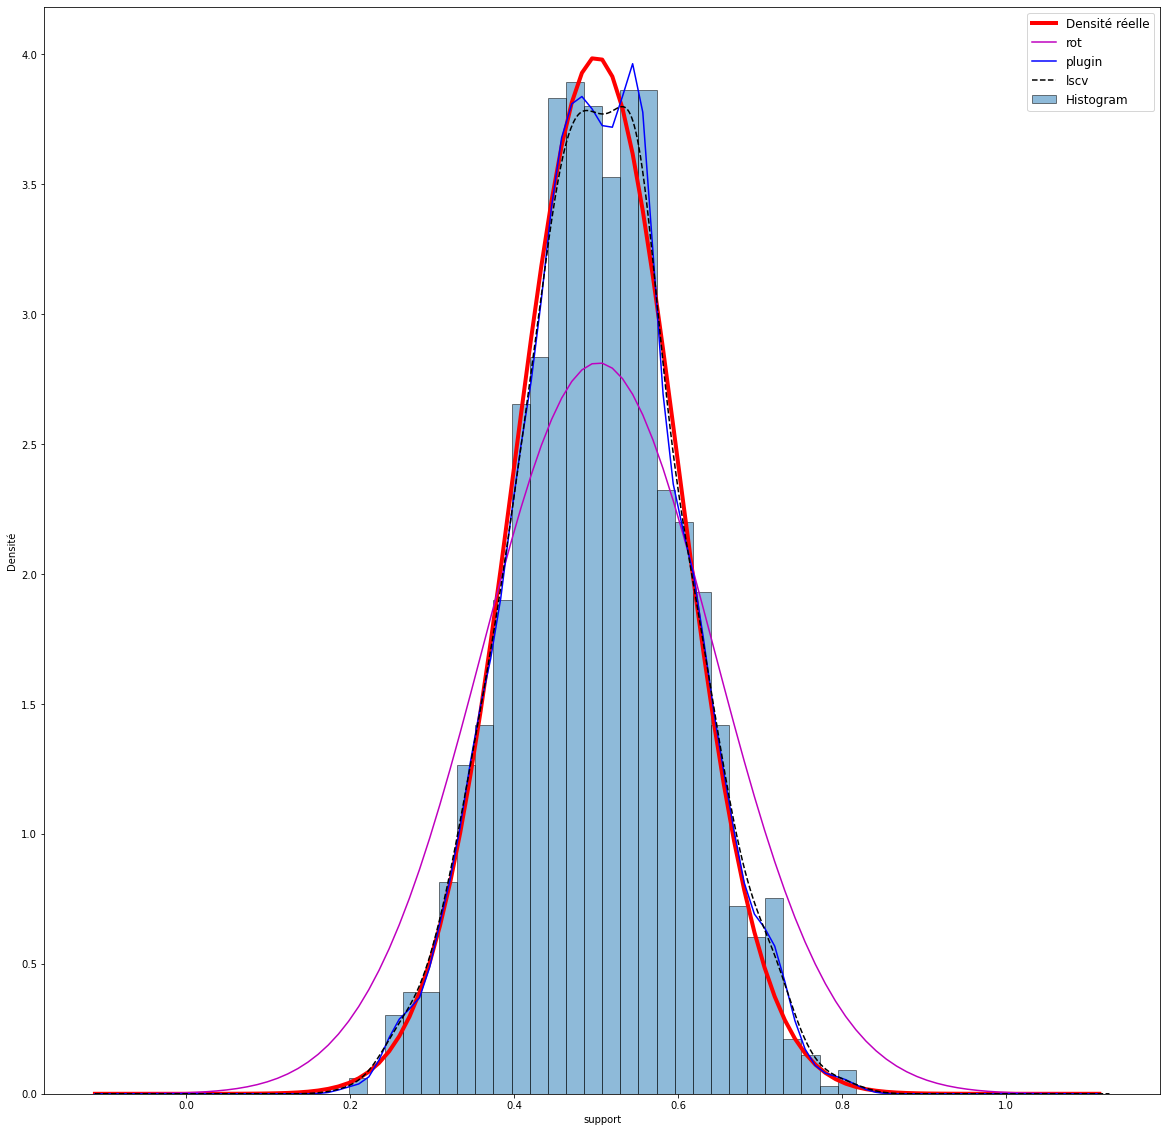
\includegraphics[width=\textwidth]{figure 3.1.png}
  \caption{Distribution G1}
  \label{fig:Différentes méthodes appliquées à la distribution G1}
\end{figure}
En observant la figure 3.1, nous pouvons constater que la méthode de l'histogramme présente des limitations en termes de précision de l'estimation de densité. Les rectangles utilisés pour représenter les classes de données introduisent des marges d'erreur, ce qui peut conduire à des estimations moins précises. Donc nous pouvons éliminer la méthode de l'histogramme dans la suite des simulations.
\clearpage
\begin{figure}[!h]
  \centering
  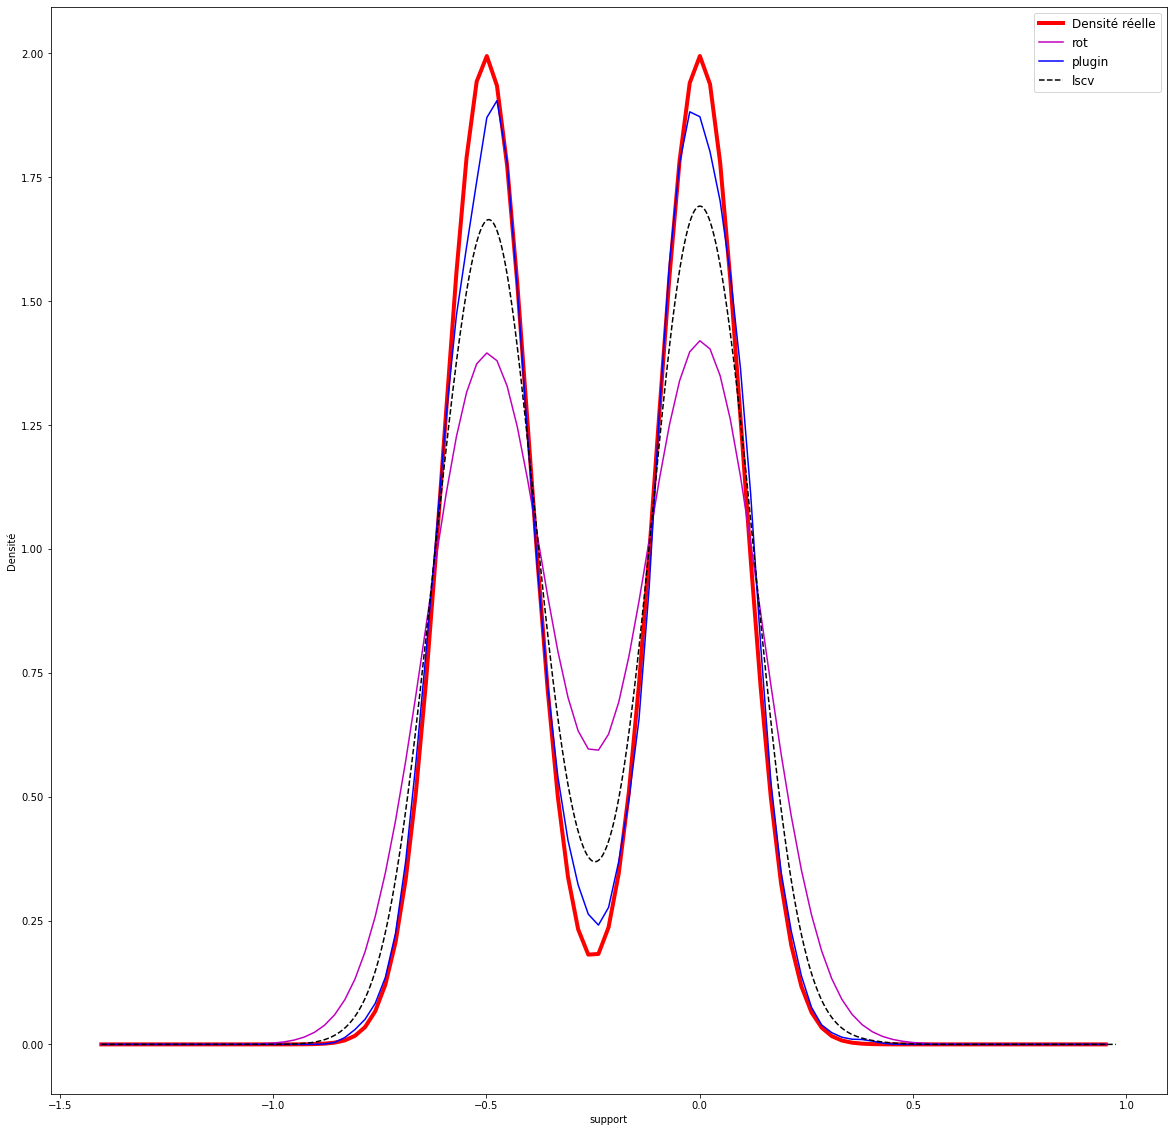
\includegraphics[width=\textwidth]{figure 3.2.png }
  \caption{Distribution G2}
  \label{fig:Différentes méthodes appliquées à la distribution G2}
\end{figure}
En examinant attentivement la figure 3.2, la méthode ROT semble produire des estimations moins précises par rapport aux méthodes LSCV  et PLUG-IN. Il est donc justifié d'éliminer la méthode ROT de nos simulations ultérieures et de poursuivre notre exploration avec les méthodes LSCV et PLUG-IN. 
\clearpage
\begin{figure}[!h]
  \centering
  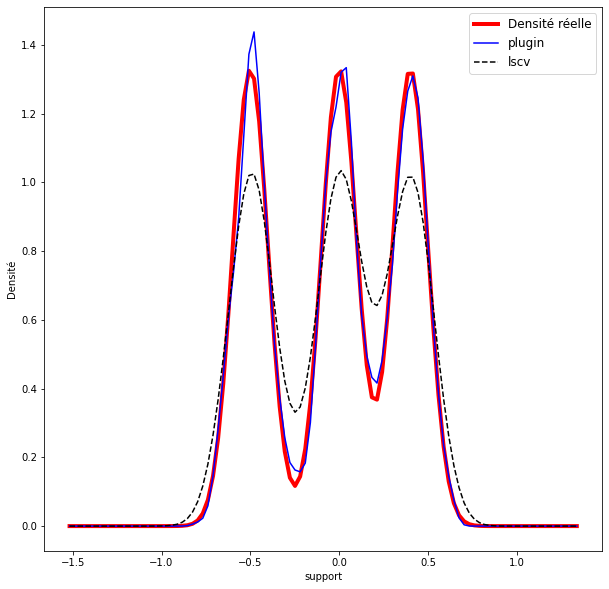
\includegraphics[width=\textwidth]{figure 3.3.png}
  \caption{Distribution G3}
  \label{fig:Différentes méthodes appliquées à la distribution G3}
\end{figure}
\clearpage
\begin{figure}[!h]
  \centering
  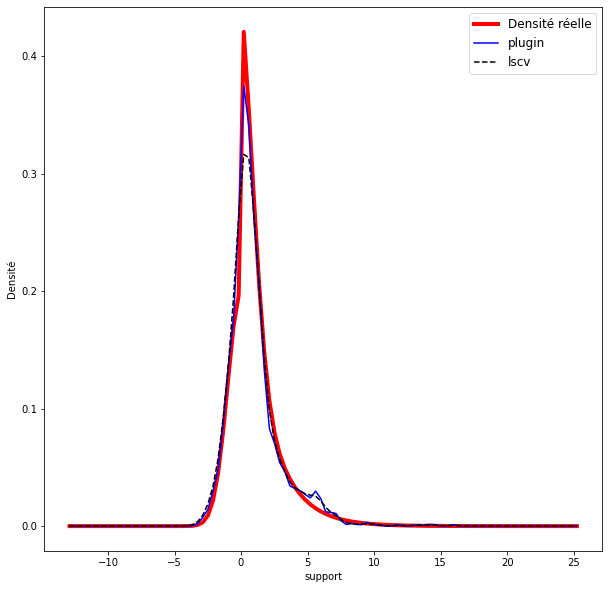
\includegraphics[width=\textwidth]{figure 3.4.png}
  \caption{Distribution G4}
  \label{fig:Différentes méthodes appliquées à la distribution G4}
\end{figure}
En analysant les deux figure 3.3 et 3.4, pour des distributions plus complexes, il devient évident que la méthode PLUG-IN produit des estimations plus précises que la méthode LSCV.
\clearpage
\begin{figure}[!h]
  \centering
  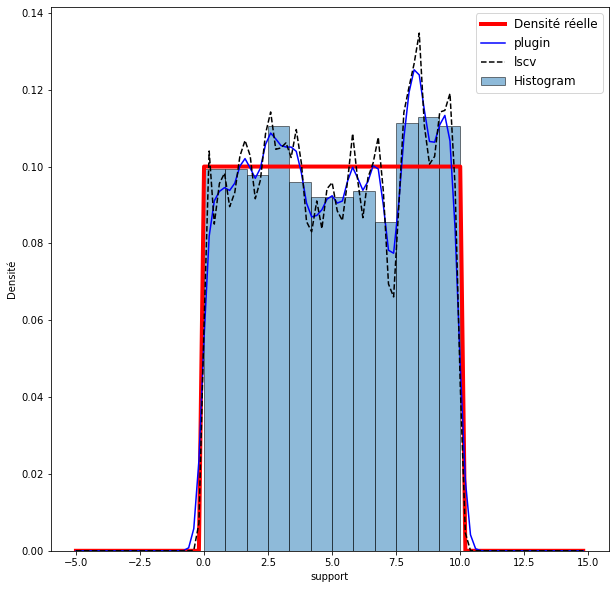
\includegraphics[width=\textwidth]{figure 3.5.png}
  \caption{Distribution G5}
  \label{fig:Différentes méthodes appliquées à la distribution G5}
\end{figure}
Lors de la simulation d'une loi uniforme (G5), nous avons remarqué que la méthode de l'histogramme peut fournir des estimations raisonnables de la densité. Les rectangles utilisés dans l'histogramme peuvent bien représenter la distribution uniforme, ce qui conduit à des estimations relativement précises. Cependant, en consultant les tables 3.1, 3.2, 3.3 et 3.4, nous avons remarqué que pour la distribution G5 avec un échantillon de taille 1500, la méthode PLUG-IN présente le plus faible EQM.

Les figures dans la page suivante présentent évolution EQM par taille d'échantillon pour différentes méthodes pour les 5 distributions (G1...G5) :  
\begin{figure}[!h]
  \centering
  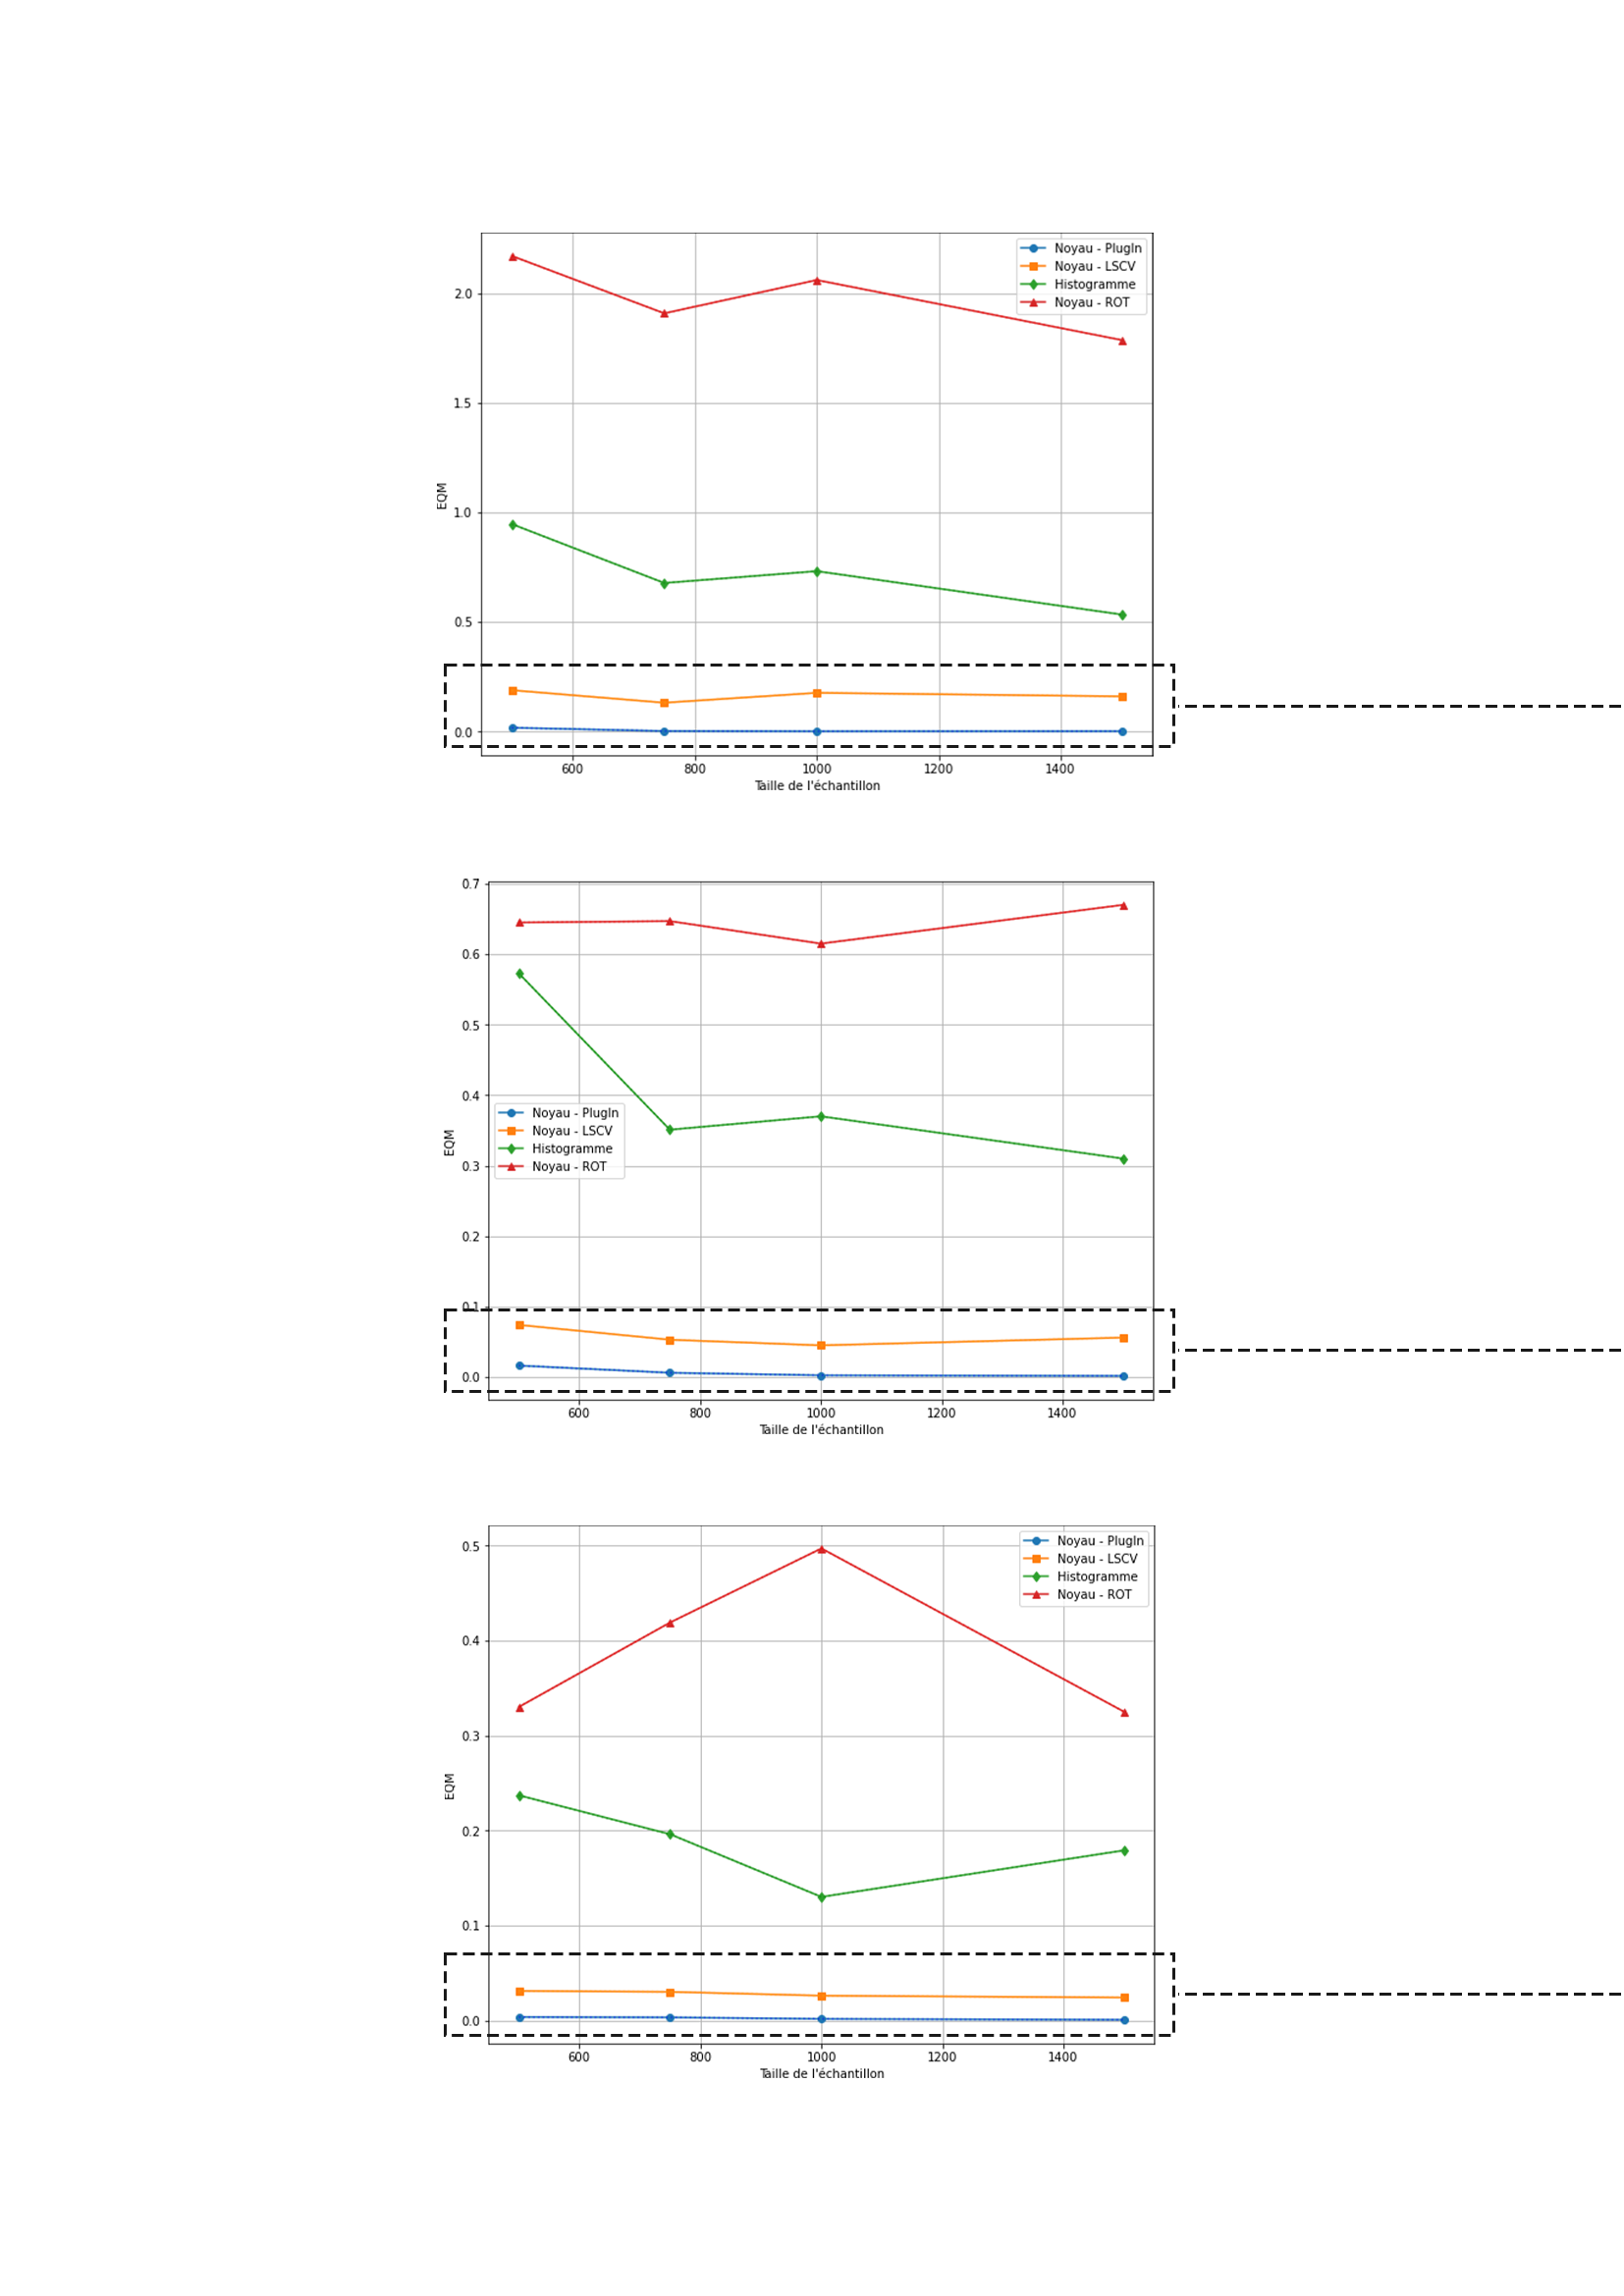
\includegraphics[width=\textwidth]{P 01.png}
  \caption{EQM : G1-G2-G3}
  \label{fig:G1-G2-G3}
\end{figure}
\begin{figure}[!h]
  \centering
  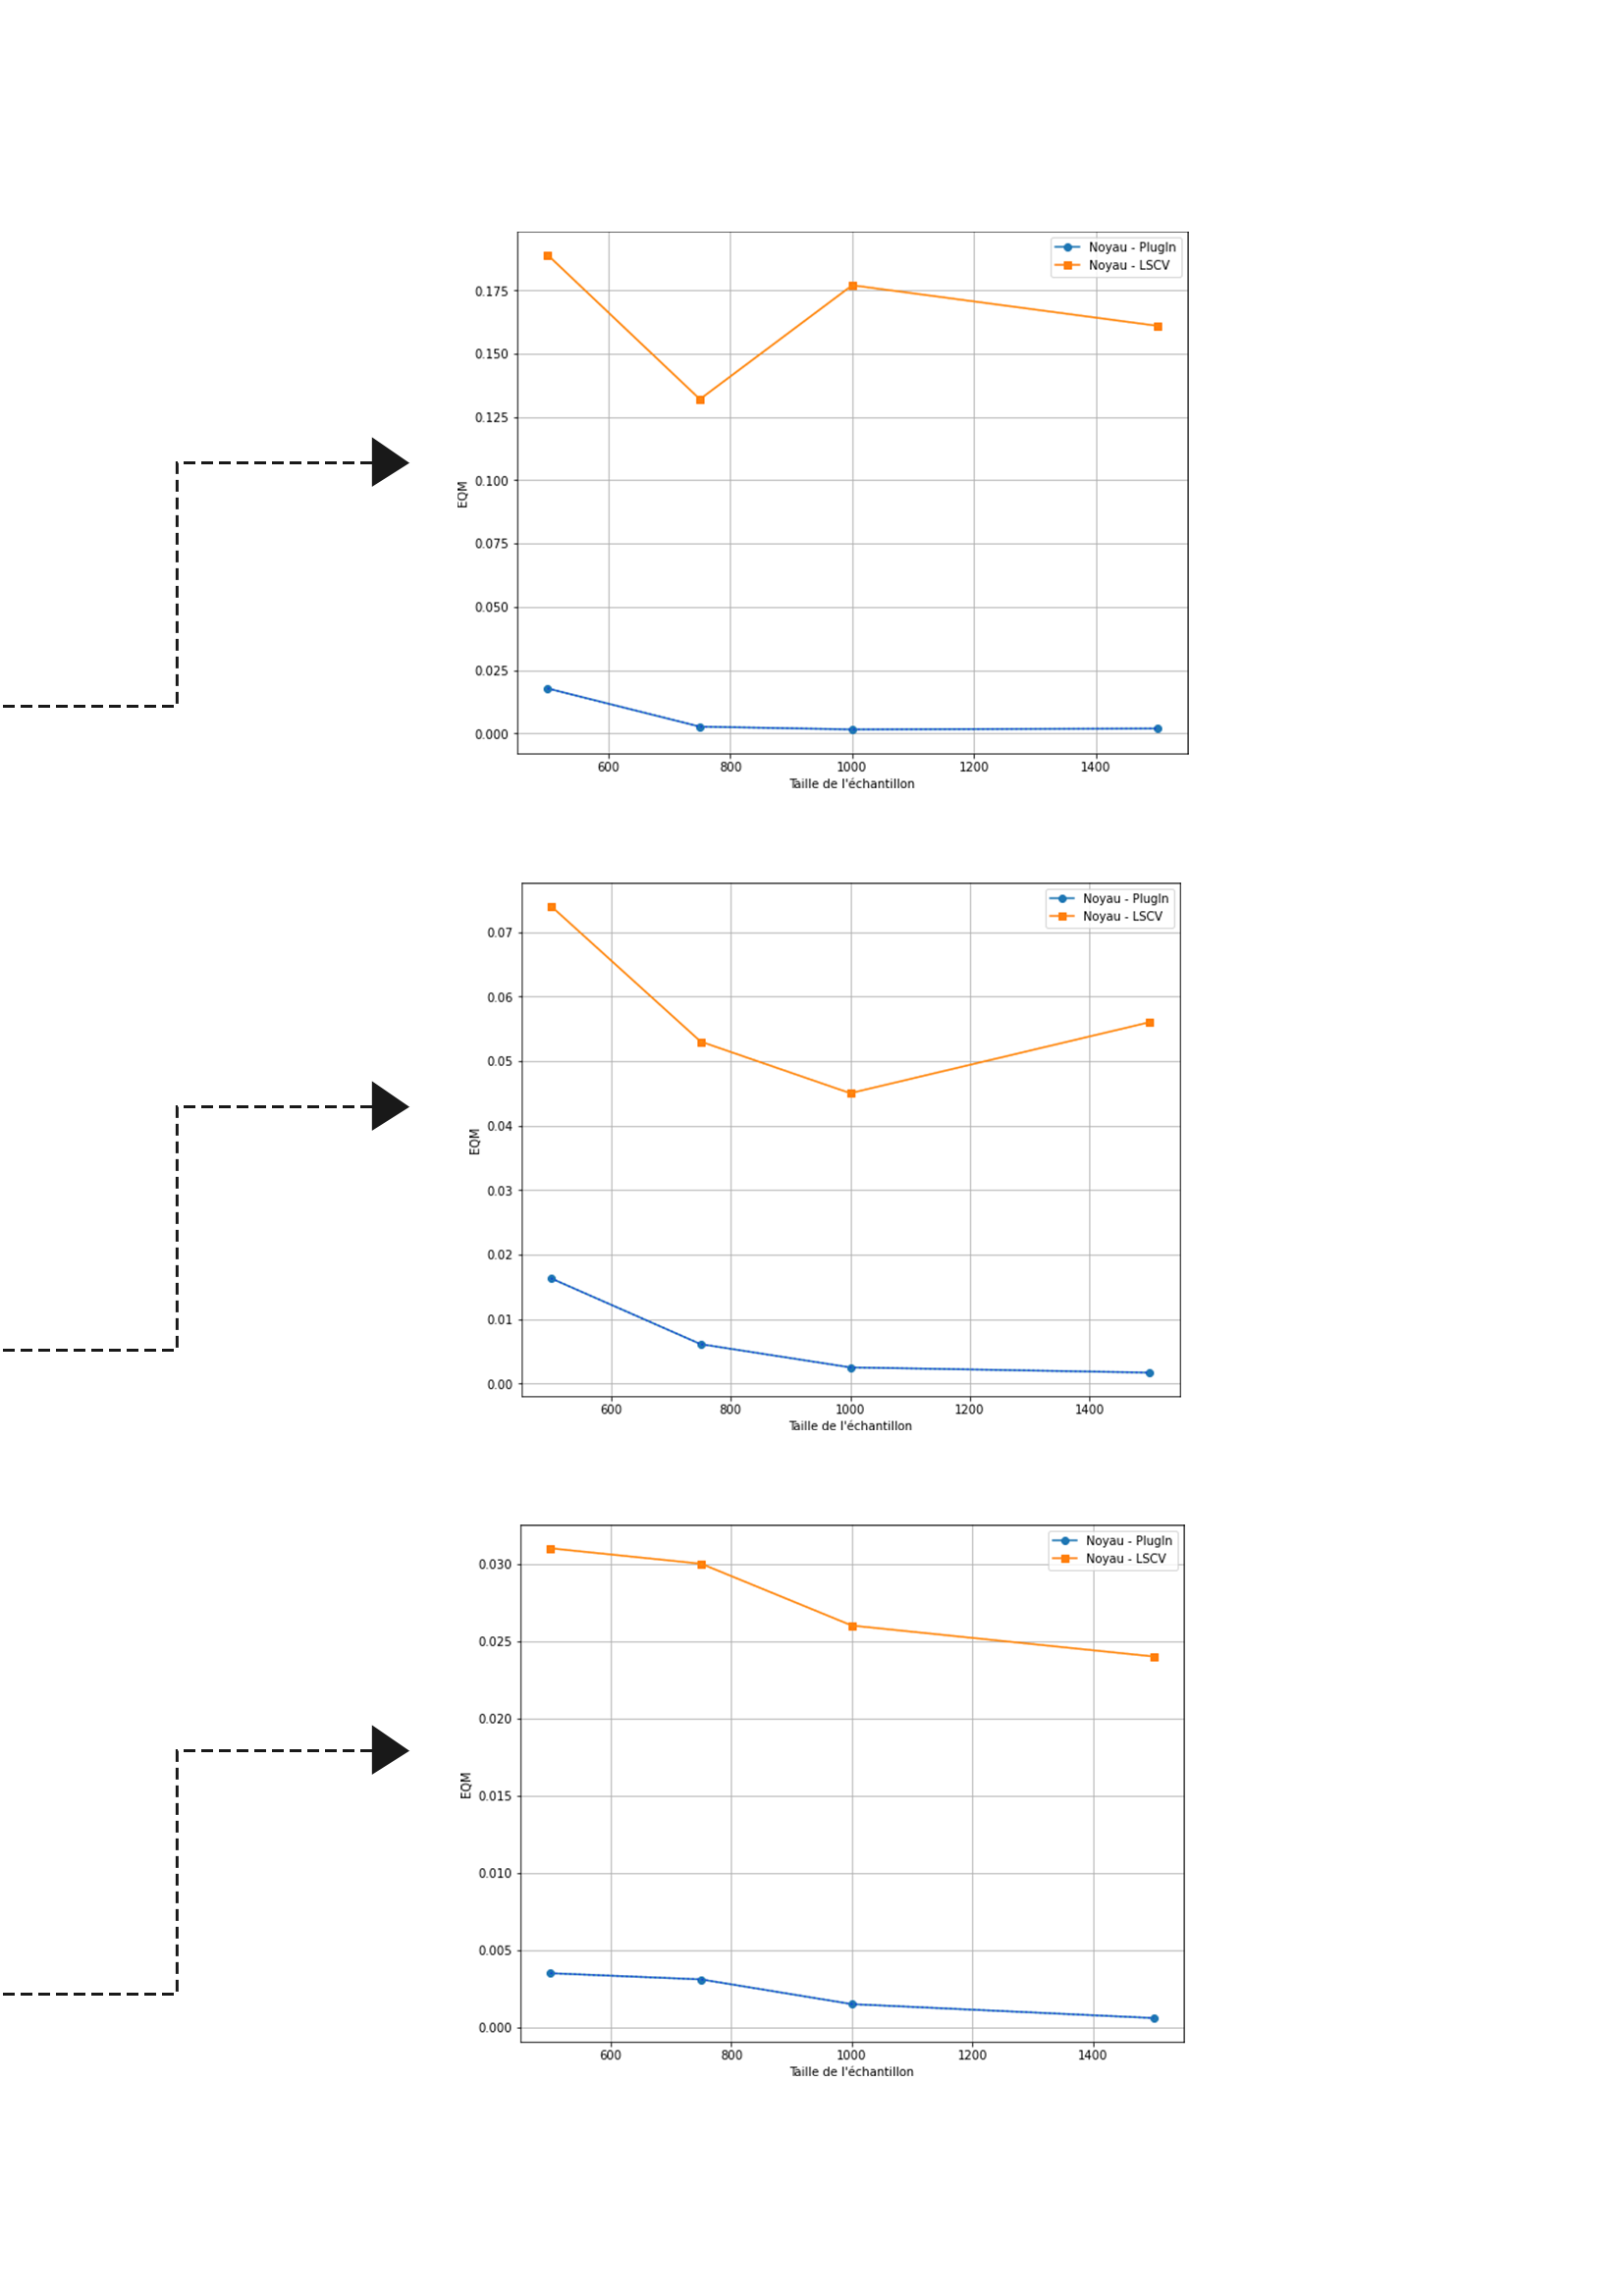
\includegraphics[width=\textwidth]{P 02.png}
  \caption{EQM : G1-G2-G3}
  \label{fig:G1-G2-G3}
\end{figure}
\begin{figure}[!h]
  \centering
  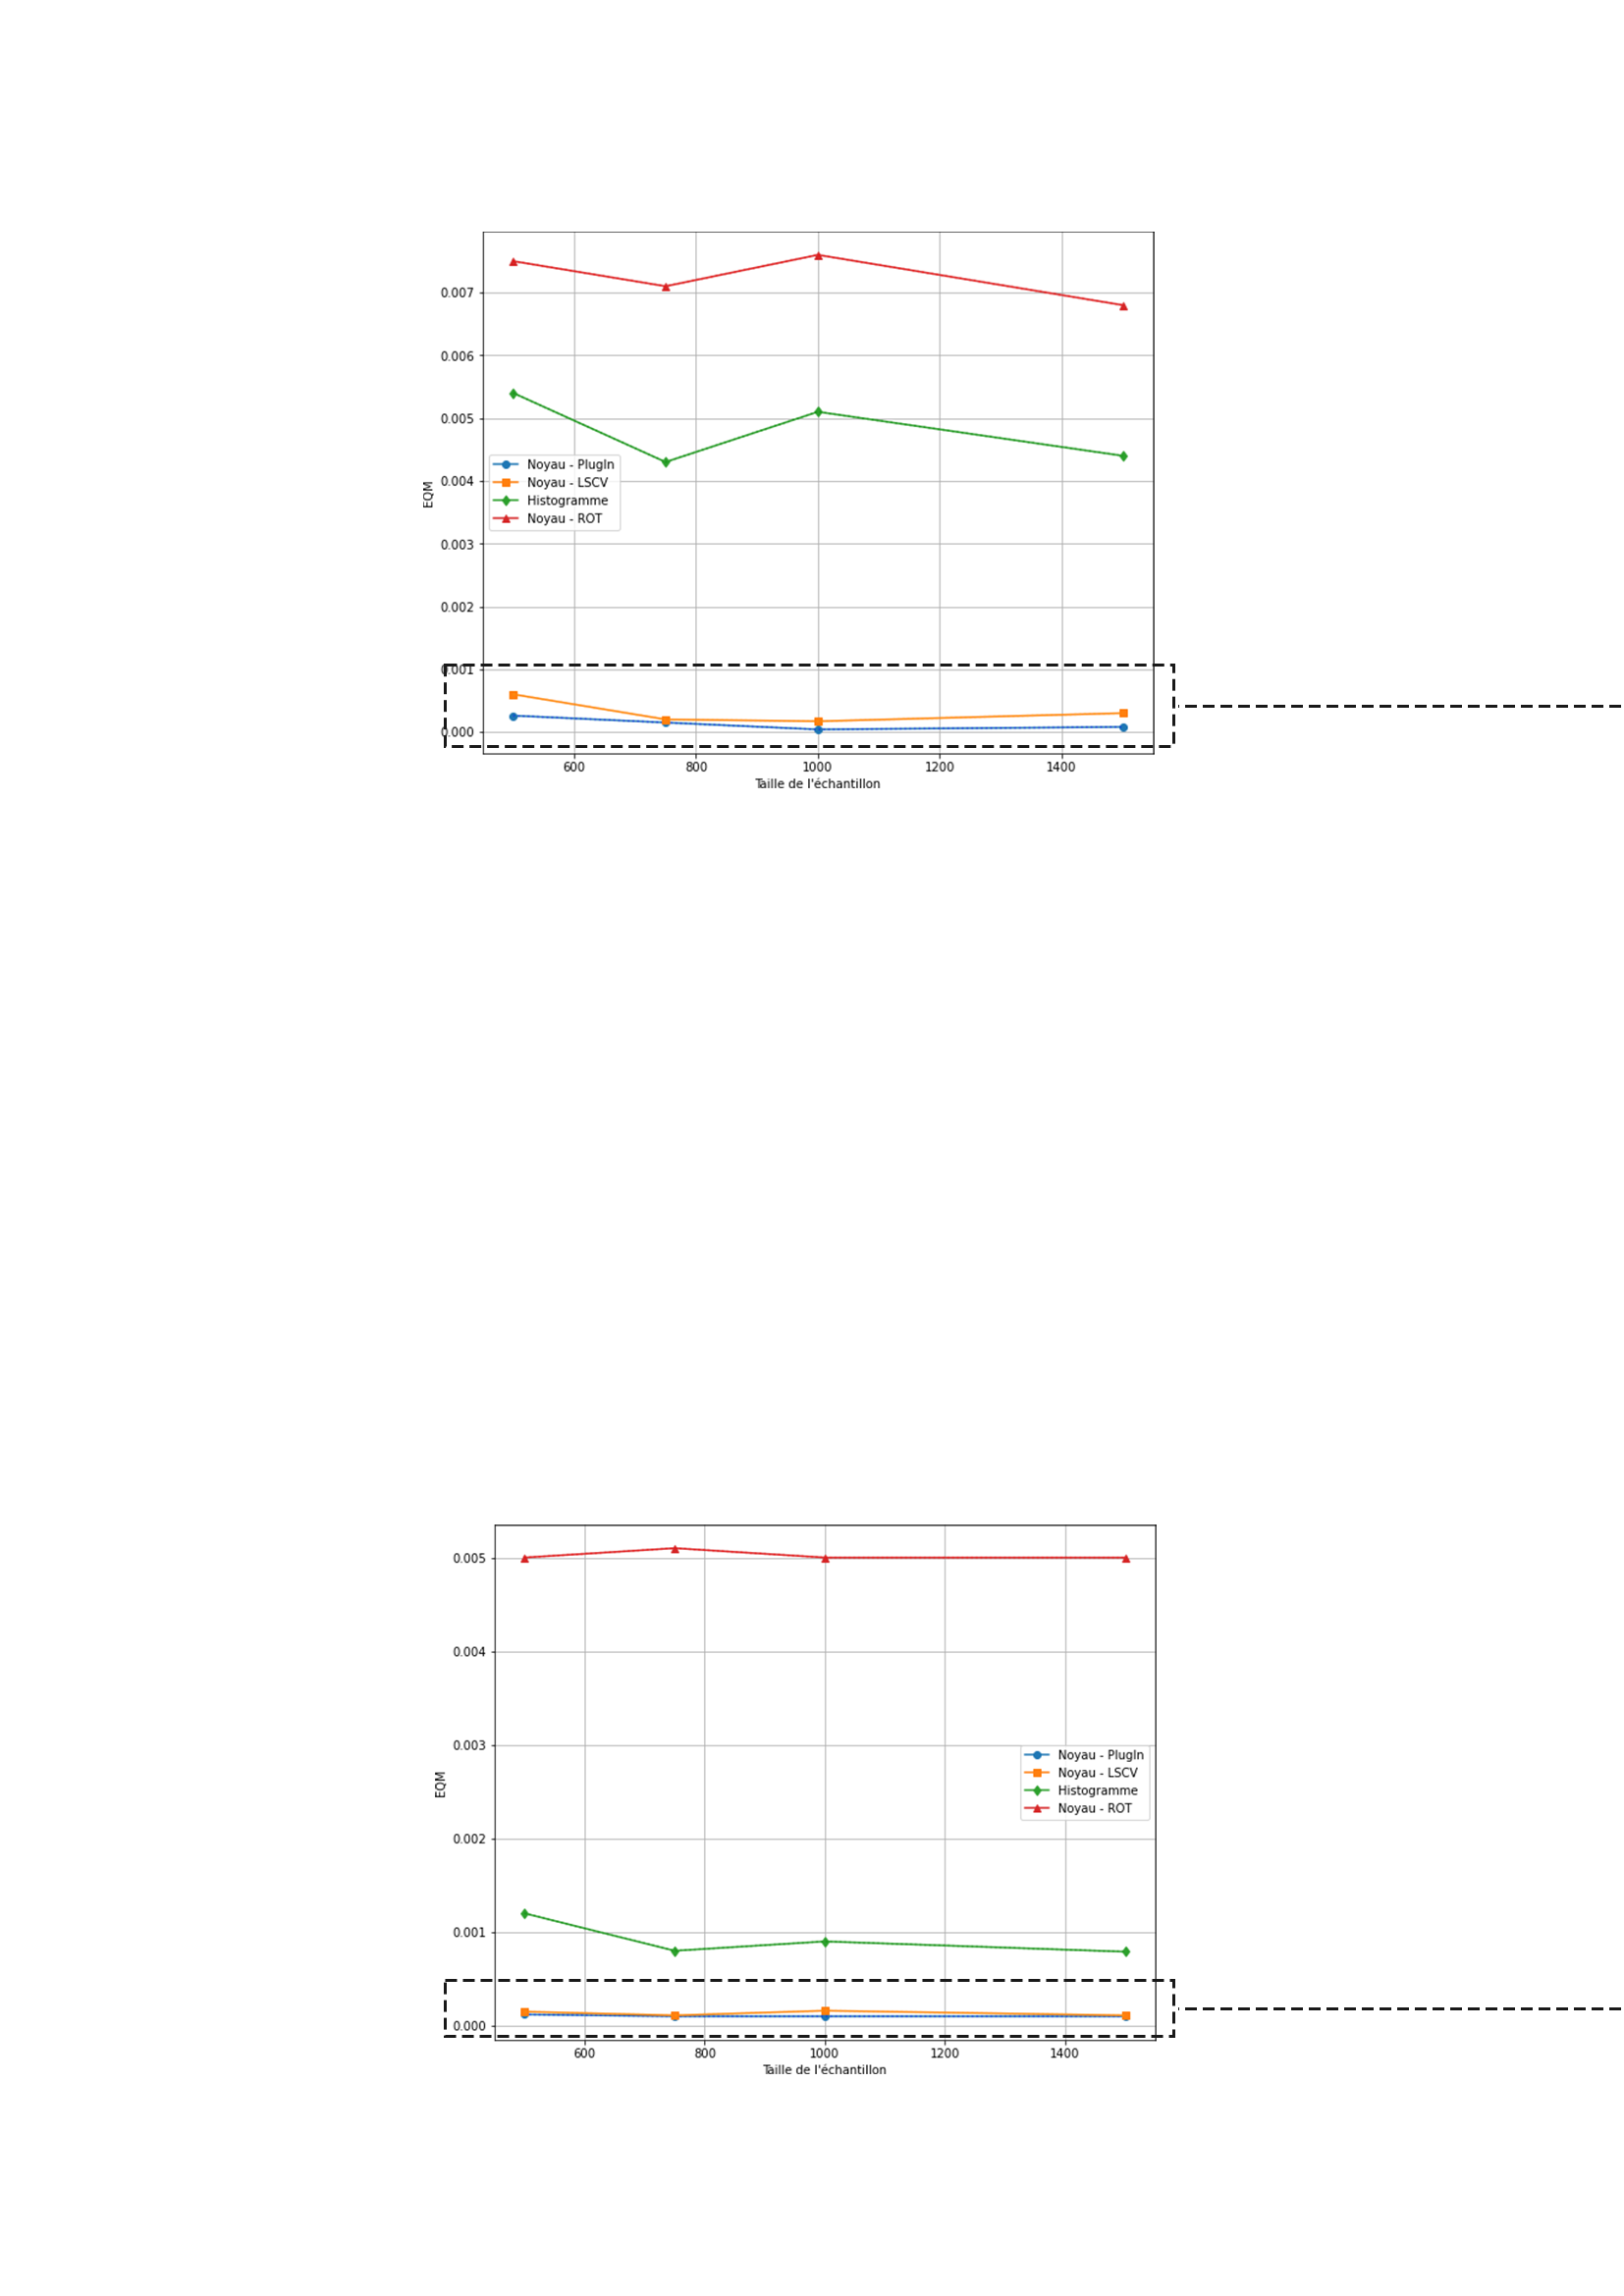
\includegraphics[width=\textwidth]{P 03.png}
  \caption{EQM  G4-G5}
  \label{fig:G4-G5}
\end{figure}
\begin{figure}[!h]
  \centering
  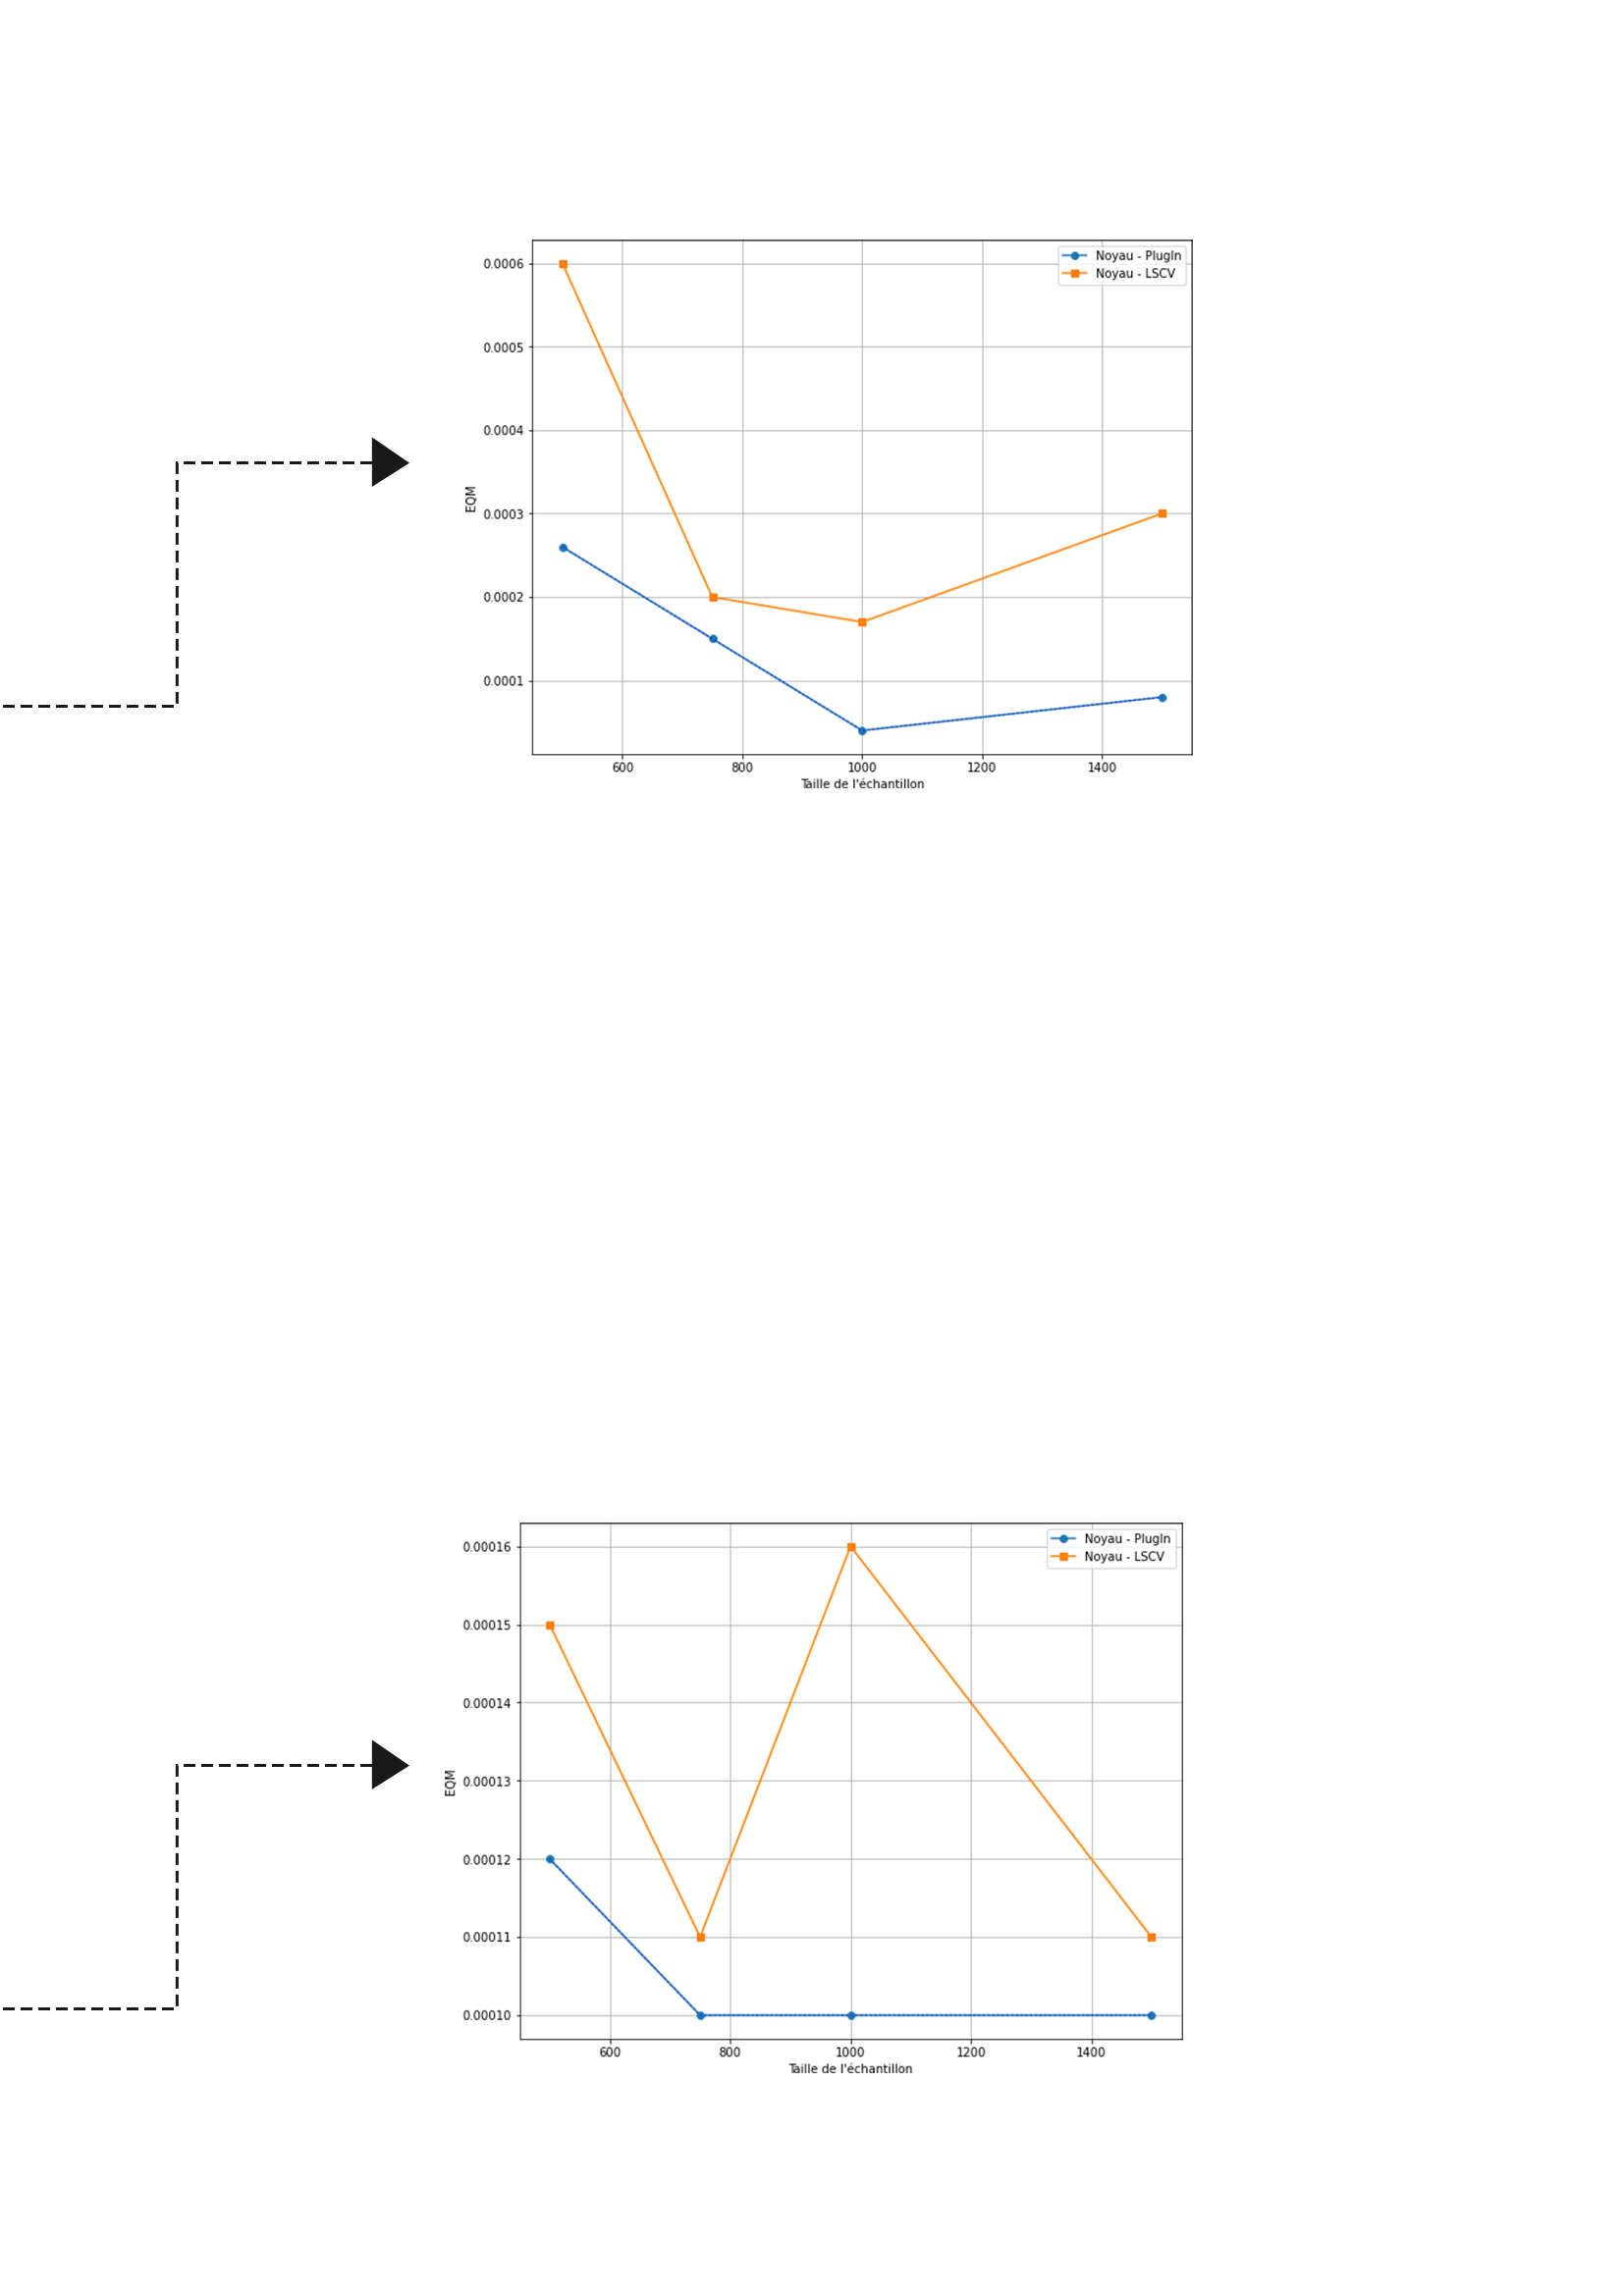
\includegraphics[width=\textwidth]{P 04.png}
  \caption{EQM : G4-G5}
  \label{fig:G1-G2-G3}
\end{figure}
\clearpage
\section{Interprétations}
L'analyse des résultats montre que la méthode de Plug-in noyau présente des performances généralement supérieures aux autres méthodes en termes d'erreur quadratique moyenne (EQM) pour les cinq distributions étudiées. Cela peut s'expliquer par le fait que la méthode de Plug-in noyau utilise une estimation non paramétrique de la ddp en ajustant un noyau à chaque point de données, ce qui peut permettre de mieux capturer la structure sous-jacente de la distribution réelle. En revanche, les autres méthodes telles que la méthode ROT, qui est implémentée par défaut en Python, peuvent avoir des limitations dans la capacité à estimer avec précision les densités de probabilité pour des distributions complexes ou multimodales.
 
Il est intéressant de noter que pour les distributions de type loi normale, l'EQM diminue au fur et à mesure que l'on passe d'une distribution uni-modale à une distribution bi ou tri modale pour les méthodes d'optimisation de paramètre de lissage. Cela peut s'expliquer par le fait que les distributions bimodales ou tri-modales présentent des caractéristiques plus complexes avec des pics multiples, ce qui peut rendre l'estimation de la ddp plus difficile pour certaines méthodes. Cependant, l'algorithme de Plug-in semble mieux s'ajuster au pas optimal des distributions complexes, permettant d'atteindre des EQM plus faibles.

Il est également intéressant de noter que la taille de l'échantillon semble jouer un rôle important dans la précision des estimations. En effet, l'EQM diminue généralement avec l'augmentation de la taille de l'échantillon pour les simulations étudiées. En effet, des échantillons plus grands permettent d'obtenir plus d'information sur la distribution réelle et permettent ainsi d'obtenir des estimations plus précises de la ddp.

En ce qui concerne la comparaison entre la méthode de Plug-in noyau et la méthode LSCV,  ces deux méthodes présentent des performances similaires, pour les distributions uni-modales cependant un EQM toujours légèrement supérieur pour l'algorithme plug-in 

Enfin, la méthode de l'histogramme présente de bonnes performances en termes d'EQM pour toutes les distributions étudiées, tout en étant simple à implémenter. Bien que l'histogramme puisse présenter des limitations en termes de résolution et de lissage de la distribution, notamment pour les distributions complexes, il peut être suffisamment précis pour des distributions plus simples et présenter un bon compromis entre simplicité d'implémentation et précision des estimations.

En conclusion, les résultats obtenus montrent que la méthode de Plug-in noyau est généralement meilleure en termes d'EQM par rapport aux autres méthodes étudiées, notamment pour les distributions tri-modales. Cependant, la taille de l'échantillon et la complexité de la distribution peuvent également jouer un rôle important dans la précision des estimations. La méthode LSCV présente des performances similaires à la méthode de Plug-in noyau, mais peut sous-estimer la complexité de la distribution réelle. La méthode de l'histogramme présente également de bonnes performances en termes d'EQM pour certaines distributions notamment la loi uniforme, tout en étant simple à implémenter. Enfin, il est important de noter que le choix de la méthode d'estimation de densité de probabilité dépendra des caractéristiques spécifiques de la distribution étudiée, de la taille de l'échantillon disponible, ainsi que des objectifs de l'analyse statistique ou de la modélisation.

Donc on peut dire que la méthode noyau Plug-in est la plus précise et la plus robuste.

\section{Conclusion}
Dans ce chapitre, nous avons examiné plusieurs méthodes non paramétriques d'estimation de densité de probabilité et avons comparé leurs performances à l'aide de simulations pour cinq distributions différentes. Les résultats montrent que la méthode noyau Plug-in est la plus précise et la plus robuste pour estimer les densités de probabilité pour les distributions étudiées. Les méthodes LSCV, histogramme et ROT ont également donné des résultats satisfaisants, mais avec des degrés de précision différents en fonction de la distribution.

Ces résultats montrent que les méthodes non paramétriques sont des outils utiles pour estimer les densités de probabilité, en particulier lorsque la distribution est inconnue ou ne peut pas être décrite par une distribution paramétrique. Cependant, il est important de choisir la méthode appropriée en fonction de la précision souhaitée et de la robustesse aux différentes formes de distribution.

En conclusion, la méthode noyau Plug-in est la méthode la plus précise et la plus robuste, mais les autres méthodes peuvent également être utilisées avec des résultats satisfaisants, en fonction de la distribution et de l'objectif de l'analyse.
\newpage
\thispagestyle{empty}
\null\newpage

